\documentclass{mwhittaker}
\title{Bipartisan Paxos}

\usepackage{pervasives}
\usepackage{tikz}
\usetikzlibrary{calc}
\usetikzlibrary{shapes.misc}

\begin{document}
\maketitle

\section{Overview}
Egalitarian Paxos~\cite{moraru2013there}, or EPaxos, is a state machine
replication protocol, like Raft~\cite{ongaro2014search} or Viewstamped
Replication~\cite{liskov2012viewstamped}. An EPaxos instance consists of a
fixed set of $n = 2f + 1$ nodes, where $f$ denotes the maximum allowable number
of node failures. With EPaxos, clients forward state machine commands to one of
the $n$ nodes. When a node receives a command $a$ from a client, it can get the
command $a$ chosen after one round trip of communication to a superquorum of
the $n$ nodes if no other concurrently proposed command conflicts with $a$. If
there is a concurrently proposed command that conflicts with $a$, then the node
can get $a$ chosen after potentially one additional round trip of communication
to a quorum (just a quorum, not a superquorum) of the $n$ nodes.

EPaxos has a number of nice features that set it apart from other state machine
replication protocols. For example, it can choose non-conflicting commands in
one round trip, disjoint sets of conflicting commands do not affect each other,
and superquorum sizes are one node smaller than the superquorum sizes used by
other protocols. The only bad thing about EPaxos is its complexity. It's not
easy to understand why EPaxos is correct.
%
In this paper, we describe a slight variant of EPaxos called Bipartisan Paxos,
or BPaxos. BPaxos retains almost all of the nice properties of EPaxos (BPaxos'
superquorum size is one larger than that of EPaxos) but is simpler to
understand.

\section{Bipartisan Paxos}
In this section, we describe BPaxos. We initially describe BPaxos as a simple
protocol that is very easy to understand, but not at all efficient. We then
repeatedly tweak the protocol. Every tweak makes the protocol more efficient,
and the tweaks also preserve the correctness of the protocol in a (hopefully)
obvious way. When we're finished tweaking, we end up with a protocol that has
almost the same performance guarantees as EPaxos.
%
We'll also warn you right now that we assume you have a good understanding of
Fast Paxos~\cite{lamport2006fast}. If you don't, the tweaks are not going to
make any sense.

\subsection{A Simple Protocol}
Recall that the EPaxos protocol is divided into two main components. The first
component constructs a directed graph of state machine commands and decides
when certain commands are considered \defword{committed}. The second component
executes the commands in reverse topological order one strongly connected
component at a time. BPaxos steals the second component, the command execution
component, from EPaxos without any modifications. The two algorithms execute
commands in 100\% the same way. Where BPaxos differs from EPaxos is in how it
constructs the graph and decides when commands in the graph are committed.

Our simple variant of BPaxos is illustrated in \figref{SimpleBPaxos}. A BPaxos
instance has three main components: an ordering service, a consensus service,
and a set of BPaxos nodes. We explain each of these three components in turn.

{\begin{figure}[ht]
  \centering

  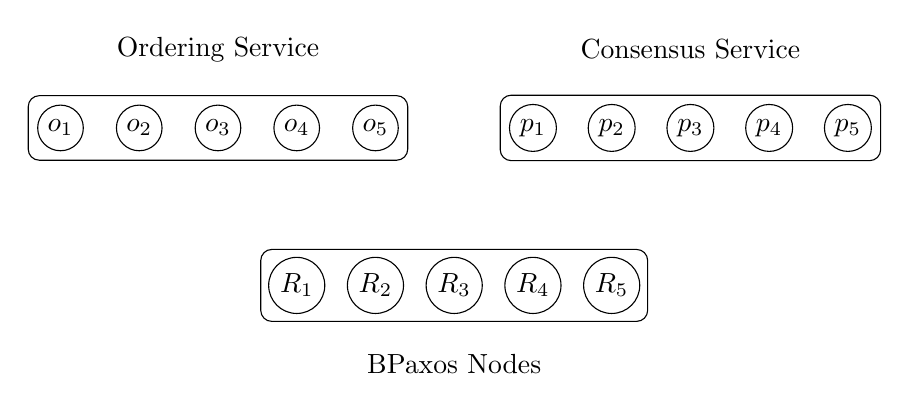
\begin{tikzpicture}
    \tikzstyle{machine}=[draw, circle, inner sep=2pt]

    % Ordering Service
    \node[machine] (o1) at (0, 2) {$o_1$};
    \node[machine] (o2) at (1, 2) {$o_2$};
    \node[machine] (o3) at (2, 2) {$o_3$};
    \node[machine] (o4) at (3, 2) {$o_4$};
    \node[machine] (o5) at (4, 2) {$o_5$};
    \node (os) at (2, 3) {Ordering Service};
    \draw[rounded corners]
      ($(o1.south west) + (-0.2, -0.2)$) rectangle
      ($(o5.north east) + (0.2, 0.2)$);

    % Consensus
    \node[machine] (p1) at (6, 2) {$p_1$};
    \node[machine] (p2) at (7, 2) {$p_2$};
    \node[machine] (p3) at (8, 2) {$p_3$};
    \node[machine] (p4) at (9, 2) {$p_4$};
    \node[machine] (p5) at (10, 2) {$p_5$};
    \node (os) at (8, 3) {Consensus Service};
    \draw[rounded corners]
      ($(p1.south west) + (-0.2, -0.2)$) rectangle
      ($(p5.north east) + (0.2, 0.2)$);

    % BPaxos Nodes
    \node[machine] (b1) at (3, 0) {$R_1$};
    \node[machine] (b2) at (4, 0) {$R_2$};
    \node[machine] (b3) at (5, 0) {$R_3$};
    \node[machine] (b4) at (6, 0) {$R_4$};
    \node[machine] (b5) at (7, 0) {$R_5$};
    \draw[rounded corners]
      ($(b1.south west) + (-0.2, -0.2)$) rectangle
      ($(b5.north east) + (0.2, 0.2)$);
    \node (bpaxos) at (5, -1) {BPaxos Nodes};
  \end{tikzpicture}

  \caption{Simple BPaxos}\figlabel{SimpleBPaxos}
\end{figure}
}

\paragraph{Ordering Service}
\newcommand{\deps}[1]{\text{deps}(#1)}

First up, the \defword{ordering service}. BPaxos nodes send state machine
commands to the ordering service. When the ordering service receives a command
$a$, it replies with a tuple $(a, \deps{a})$ where $a$ is the command and
$\deps{a} = \set{c_1, \ldots, c_n}$ is a set of commands that we call $a$'s
\defword{dependencies}. The ordering service provides the following guarantee.
If two conflicting commands $a$ and $b$ yield responses $(a, \deps{a})$ and $(b,
\deps{b})$ from the ordering service, then either $a \in \deps{b}$ or $b \in
\deps{a}$ (or both). That is, if two conflicting commands are sent to the
ordering service, at least one is guaranteed to be a dependency of the other.

Implementing a fault tolerant ordering service is straightforward. We employ
$2f + 1$ ordering service nodes $o_{1}, \ldots, o_{2f + 1}$. When a BPaxos node
sends a command $a$ to the ordering service, it sends the command to all $2f +
1$ of the ordering service nodes. Every ordering service node $o_i$ maintains a
set $C_i$ of all the commands that it has received. When node $o_i$ receives a
command $a$ from a BPaxos node, it atomically performs two actions. First,
$o_i$ replies to the BPaxos node with the pair $(a, \deps{a}_i)$ where
$\deps{a}_i = \setst{c \in C_i}{\text{$a$ and $c$ conflict}}$ is the set of
commands that $o_i$ has previously received that conflict with $a$. Second,
$o_i$ adds $a$ to $C_i$. When a BPaxos node receives replies $(a,
\deps{a}_{i_1}), \ldots, (a, \deps{a}_{i_{f+1}})$ from a quorum $Q_a$ of $f +
1$ ordering service nodes, it takes $(a, \deps{a}_{i_1} \cup \ldots \cup
\deps{a}_{i_{f+1}}) = (a, \deps{a})$ to be the response from the ordering
service.

To understand why this ordering service implementation provides its advertised
guarantees, consider conflicting commands $a$ and $b$. Assume $a$'s reply $(a,
\deps{a})$ was formed from a quorum $Q_a$ and $b$'s reply $(b, \deps{b})$ was
formed from a quorum $Q_b$. Any two quorums intersect, so $Q_a \cap Q_b$ is
nonempty. Let $o_i$ be an ordering service node in this intersection. $o_i$
either received $a$ or $b$ first. If it received $a$ first, then $a$ is in
$C_i$ when $o_i$ processed command $b$, so $o_i$ includes $a$ in $\deps{b}_i$,
so $a$ is in $\deps{b}$. Symmetrically, if $o_i$ received $b$ first, then it
includes $b$ in $\deps{a}$.

\paragraph{Consensus Service}
Next up, the \defword{consensus service}. We assume we have some set $p_1,
\ldots, p_n$ of nodes that implement Plain Jane consensus. A BPaxos node can
propose to the consensus service that some value $v$ be chosen in some
consensus \defword{instance} $i$. The consensus service replies with the value
that has been chosen in instance $i$, which may or may not be $v$ depending on
if there are concurrent proposers proposing to instance $i$. The consensus
service guarantees that for every instance $i$, at most one value is ever
chosen in $i$.

\paragraph{BPaxos Nodes}
\newcommand{\instance}[1]{\text{inst}(#1)}

Finally, we assume a fixed set $b_1, \ldots, b_{2f+1}$ of $2f + 1$ BPaxos
nodes. Each BPaxos node $b$ manages an infinite set $\instance{b}_1,
\instance{b}_2, \instance{b}_3, \ldots$ of consensus instances.
%
Clients sends state machine commands to BPaxos nodes to be executed by the
replicated state machine. When a BPaxos node $b$ receives a command $a$, it
sends the command to the ordering service and receives a reply $(a, \deps{a})$.
$b$ then proposes the value $(a, \deps{a})$ to the consensus service in some
previously unused instance $\instance{b}_i$. The consensus service then replies
with some chosen value $(a', \deps{a'})$, which is equal to $(a, \deps{a})$ in
the failure-free case. At this point, the command $a'$ is considered committed
in the directed graph of state machine commands with inbound edges from
commands in $\deps{a'}$. Node $b$ also informs the other BPaxos nodes that the
value $(a', \deps{a'})$ has been committed. As noted earlier, the execution of
the commands in the directed graph is identical to that of EPaxos. Committed
commands are committed in reverse topological order, one strongly connected
component at a time.
% TODO: Explain no liveness.

That's the basic version of BPaxos. We can prove it's correct by leveraging
EPaxos' proof of correctness.
% TODO: Reference EPaxos proof and show our thing works.
% TODO: Show no liveness.

\subsection{Tweak 1: Paxos and Liveness}
% TODO: Implement consensus with Paxos. On failure, re-run paxos substituting
% no-ops if needed.
% TODO: Show liveness works now.

% \subsection{Tweak 2: Colocation}
% \subsection{Tweak 3: Enter Fast Paxos}
% \subsection{Tweak 4: Coordinated Recovery}

% \section{Comparison with EPaxos}
% TODO: quorum sizes + fast BPaxos.

\bibliographystyle{plain}
\bibliography{references}
\end{document}
